\documentclass[border=2pt]{standalone}
\usepackage{tikz}
\usetikzlibrary{arrows.meta,positioning,fit}
\begin{document}
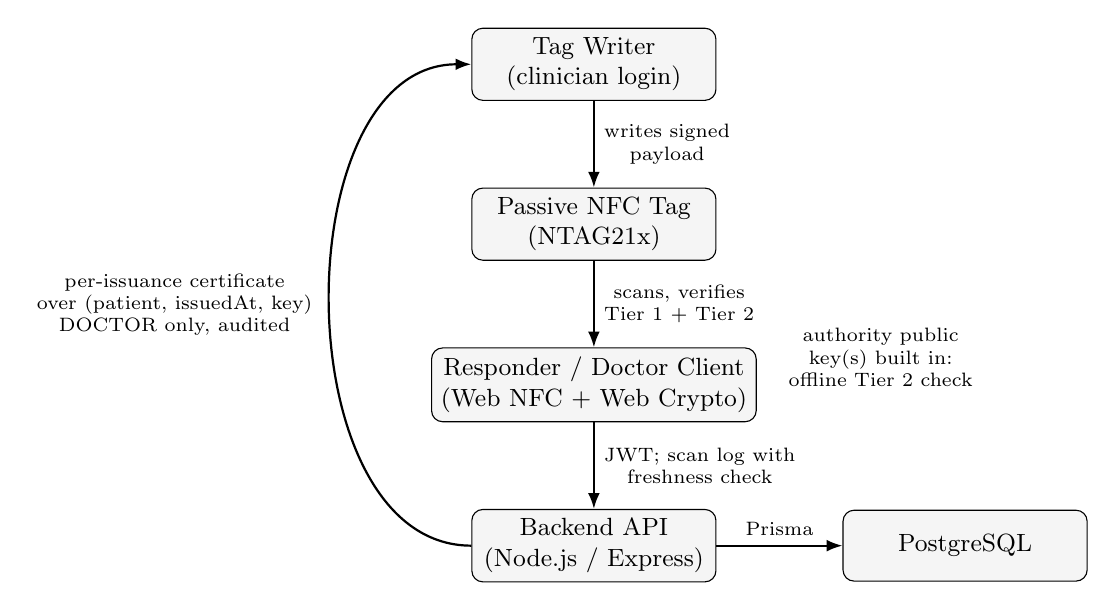
\begin{tikzpicture}[
  box/.style={draw, rounded corners, align=center, font=\small, minimum height=0.9cm, minimum width=3.1cm, fill=gray!8},
  arr/.style={-{Latex[length=2mm]}, thick},
  lbl/.style={font=\scriptsize, align=center}
]
  \node[box] (admin) {Tag Writer\\(clinician login)};
  \node[box, below=1.1cm of admin] (tag) {Passive NFC Tag\\(NTAG21x)};
  \node[box, below=1.1cm of tag] (client) {Responder / Doctor Client\\(Web NFC + Web Crypto)};
  \node[box, below=1.1cm of client] (backend) {Backend API\\(Node.js / Express)};
  \node[box, right=1.6cm of backend] (db) {PostgreSQL};

  \draw[arr] (admin) -- node[lbl, right] {writes signed\\payload} (tag);
  \draw[arr] (tag) -- node[lbl, right] {scans, verifies\\Tier 1 + Tier 2} (client);
  \draw[arr] (client) -- node[lbl, right] {JWT; scan log with\\freshness check} (backend);
  \draw[arr] (backend) -- node[lbl, above] {Prisma} (db);

  \draw[arr] (backend.west) to[out=180,in=180] node[lbl, left, xshift=-0.1cm] {per-issuance certificate\\over (patient, issuedAt, key)\\DOCTOR only, audited} (admin.west);

  \node[lbl, right=0.15cm of client, yshift=0.35cm, text width=2.6cm] {authority public\\key(s) built in:\\offline Tier 2 check};
\end{tikzpicture}
\end{document}
